\documentclass[aspectratio=1610,14pt]{beamer}
\usetheme{CSCS}

% define footer text
\newcommand{\footlinetext}{Intel KNL: Best practices and experiences}

% Select the image for the title page
\newcommand{\picturetitle}{cscs_images/image3.pdf}
%\newcommand{\picturetitle}{cscs_images/image5.pdf}
%\newcommand{\picturetitle}{cscs_images/image6.pdf}

\lstdefinestyle{cppstyle}{
  basicstyle=\ttfamily\small,
  language=[11]C++
}



% Please use the predifined colors:
% cscsred, cscsgrey, cscsgreen, cscsblue, cscsbrown, cscspurple, cscsyellow, cscsblack, cscswhite

\author{Vasileios Karakasis}
\title{Early experiences on porting NestMC to KNL using intrinsics}
\subtitle{Intel KNL: Best practices and experiences}
\date{April 6, 2017}

\begin{document}

% TITLE SLIDE
\cscstitle

\cscstableofcontents{Outline}

\section{What is NestMC?}
\subsection{Goals}
\subsection{Design and architecture}
\subsection{Critical simulation steps}
\section{Compiling channel and synapse states}
\subsection{The KNL backend}
\section{Experiences with intrinsics}
\subsection{Helpful tricks}
\subsection{Turndowns}


% Block style example
\begin{frame}{What is NestMC?}
  NestMC is a project to develop
  \begin{itemize}
  \item a new multi-compartmental neuron simulator,
  \item that is optimized for HPC systems,
  \item and is easy to integrate into existing workflows.
  \end{itemize}
\end{frame}

\begin{frame}{Who is behind the initiative?}
  \centering
  \vspace{1ex}
  {\large Cross-institutional collaboration}\\[2ex]
  % dodgy by-hand scaling
  
\includegraphics[height=2.8em]{logos/cscs_logo.pdf}
  \hspace{15mm}
  
\includegraphics[height=3em]{logos/julich_logo.pdf}
  \hspace*{5mm}
  \\[1.4em]
  
\includegraphics[height=2.9em]{logos/bsc_logo.pdf}\\

  \vfill
  {\large As part of}\\[2ex]
  
\includegraphics[height=3em]{logos/nest-initiative.pdf}
  %\\[1.4em]
  \hspace{15mm}
  
\includegraphics[height=3em]{logos/HBP_logo.jpg}
  \vspace*{1em}
\end{frame}

\begin{frame}{Limitations of current solutions}
  \begin{itemize}
  \item There are problems and models that we can't explore with current software and systems
    \begin{itemize}
    \item Near real-time multi-compartment simulations
    \item `Large' networks
    \item Field potential calculations
    \end{itemize}
  \item New HPC architectures
    \begin{itemize}
    \item Highly parallel architectures (e.g.\ Intel KNL)
    \item Wide vector operations (e.g.\  AVX512)
    \item Specialized accelerator hardware (GPUs, FPGAs)
    \end{itemize}
  \item Adapting existing simulators to new architectures is \emph{hard}
  \end{itemize}
\end{frame}

\begin{frame}{NestMC goals}
  \vfill
  \begin{columns}[t,onlytextwidth]
    \column{0.3\textwidth}
    \centering Interoperability
    \\[2ex]
    \small
    {\em Simulator as library}
    \\
    \begin{itemize}
      \small
      \setlength{\itemsep}{0.2ex}
    \item Visualization
    \item Multi-physics
    \item Multi-scale
    \end{itemize}

    \column{0.3\textwidth}
    \centering Extensibility
    \\[2ex]
    \small
    {\em Modular internal API}
    \\
    \begin{itemize}
      \small
      \setlength{\itemsep}{0.2ex}
    \item New integration schemes
    \item Custom spike communication
    \item Specialized cells
    \end{itemize}

    \column{0.3\textwidth}
    \centering Performance
    \\[2ex]
    \small
    {\em HPC targeted}
    \begin{itemize}
      \small
      \setlength{\itemsep}{0.2ex}
    \item Highly parallel
    \item GPU and vector targets
    \item Design for scalability
    \end{itemize}
  \end{columns}
  \vspace{4ex}
\end{frame}

\begin{frame}{NestMC design}
  \begin{itemize}
  \item Modular: components can be substituted according to internal API
  \item Internal API: `thin' API; type parameterization allows components to determine low-overhead API data structures
  \end{itemize}
  \begin{center}
    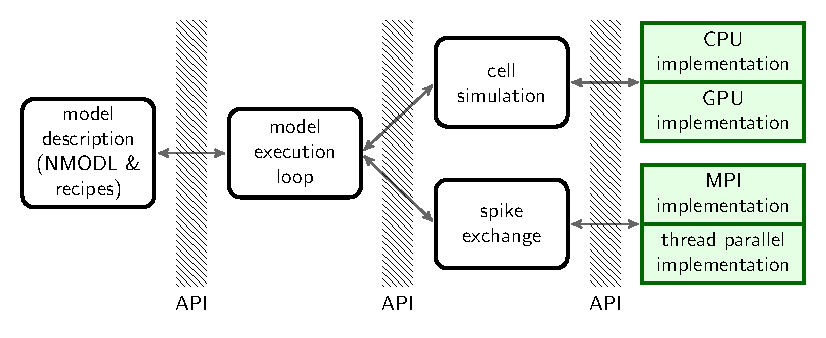
\includegraphics[width=.9\textwidth]{figs/api.pdf}
  \end{center}
\end{frame}


\begin{frame}{NestMC backends}
  Cell simulation modules share computational backends for channel and synapse state evolution.

  \vfill
  \centering
  CPU-hosted finite volume cell simulation\\
  \vspace{2ex}
  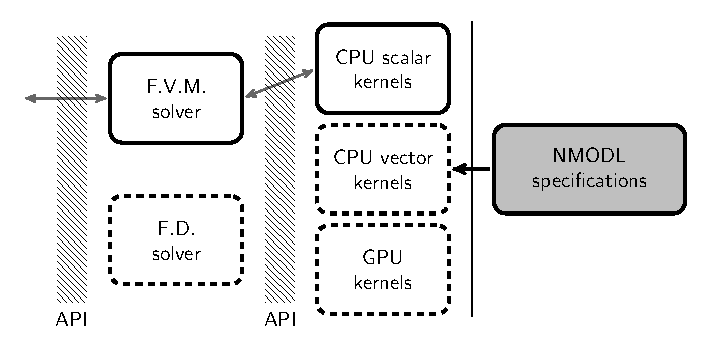
\includegraphics[height=0.5\textheight]{figs/backend-api.pdf}

  \vfill
\end{frame}

\begin{frame}{Cell simulation timeloop}
  \begin{center}
    \only<1>{
      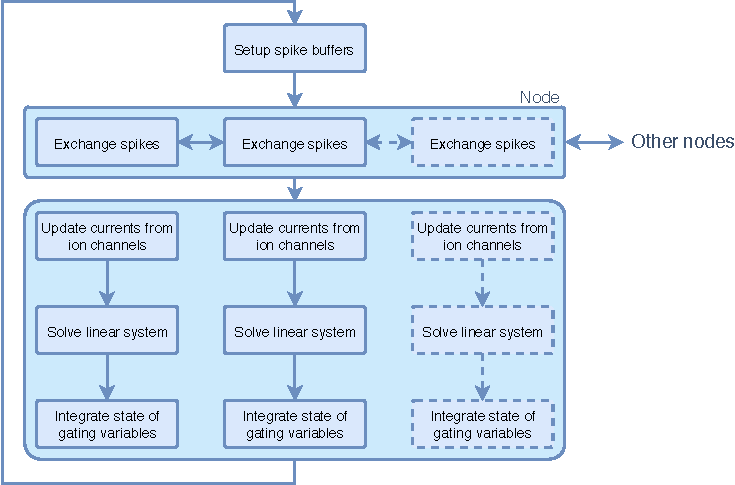
\includegraphics[height=.75\textheight]{figs/timeloop.pdf}
    }
    \only<2>{
      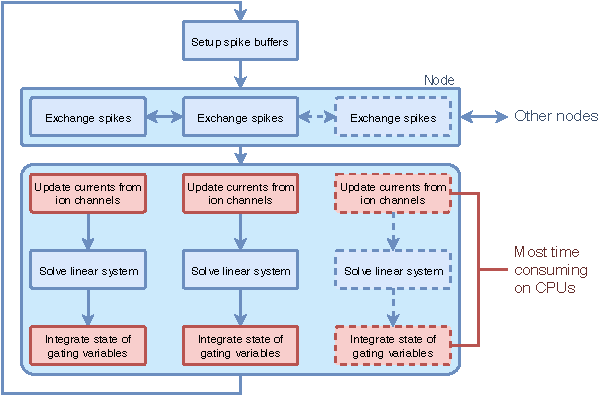
\includegraphics[height=.75\textheight]{figs/timeloop-overlay.pdf}
    }
  \end{center}
\end{frame}

\begin{frame}{Mechanisms specifications}
  \begin{itemize}
  \item Written in NMODL
    \begin{itemize}
    \item DSL for describing membrane mechanisms of neuron cells
    \item Developed for the NEURON simulator
    \end{itemize}
  \item Translated into C++ with \texttt{modcc}
    \begin{itemize}
    \item Source-to-source compiler from NMODL to C++
    \item Generates platform-dependent code for the mechanism
    \end{itemize}
  \end{itemize}
\end{frame}

\begin{frame}{The modcc architecture}
  \begin{center}
    \only<1>{
      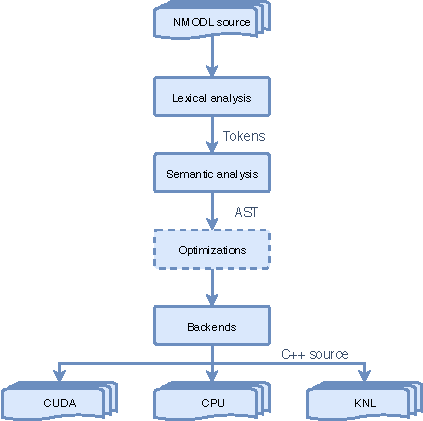
\includegraphics[height=.75\textheight]{figs/modcc.pdf}
    }
    \only<2>{
      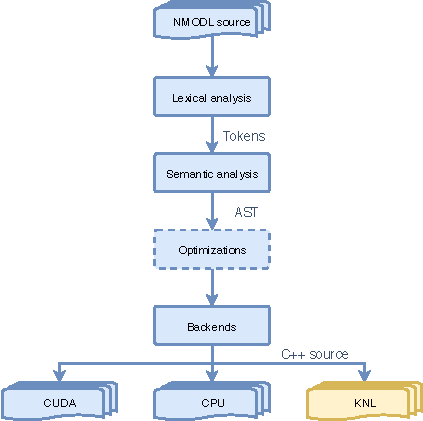
\includegraphics[height=.75\textheight]{figs/modcc-overlay.pdf}
    }
  \end{center}
\end{frame}

\begin{frame}{KNL backend -- Baseline}
  \begin{itemize}
  \item Standard CPU code, no pragmas
  \item Rely completely on compiler auto-vectorization capabilities
  \item Baseline benchmark performance: {\color{cscsred} 49.58s}
  \end{itemize}
\end{frame}

\begin{frame}{KNL backend -- Guided compiler vectorization}
  \begin{itemize}
  \item Proper alignment of data
  \item Enforce vectorization of critical loops using \texttt{\#pragma ivdep}
  \item Benchmark performance: {\color{cscsred} 19.0s (+261\%)}
  \end{itemize}
  \pause
  \vfill
  Tricky part:
  \vfill
  \begin{itemize}
  \item Some mechanisms have dependencies between vector elements
  \item Critical loops rewritten:
    \begin{itemize}
    \item Blocked on SIMD vector length
    \item Inner loop vectorized
    \item Manual accumulation of vector elements
    \end{itemize}
  \end{itemize}
\end{frame}

\begin{frame}{KNL backend -- Intrinsics}
  \begin{itemize}
  \item Original loop rewritten with intrinsics
  \item Benchmark performance: {\color{cscsred}19.5s (-2.6\%)}
    \begin{itemize}
    \item Out-of-the-box implementation, no tuning yet
    \item Unaligned memory access instructions
    \item Critical loop is different than the guided version
    \end{itemize}
  \end{itemize}
\end{frame}

\begin{frame}{KNL backend -- Intrinsics}
  Why intrinsics?
  \vfill
  \begin{itemize}
  \item We want to support also non-Intel compilers
  \item We are writing a compiler backend, so the development overhead of intrinsics is undertaken only once
  \item Don't want to depend on another high level C++ vectorization library
  \item Dive deeper in code optimizations
  \end{itemize}
\end{frame}

\begin{frame}[fragile]{Helpful tricks with intrinsics}
  Intrinsics can be chained $\rightarrow$ prefix notation
    \vfill
  \begin{Cpplisting}{\texttt{g[off\_]*(v-e[off\_])}}
_mm512_mul_pd(
    _mm512_loadu_pd(&g[off_]),
    _mm512_sub_pd(
        v, _mm512_loadu_pd(&e[off_])
    )
)
  \end{Cpplisting}
\end{frame}

\begin{frame}[fragile]{Helpful tricks with intrinsics}
  Indirect accesses through gathers and scatters
  \vfill
  \begin{Cpplisting}{\texttt{v = arr[ni[off\_]]}}
__m256i vni=_mm256_lddqu_si256(
    (const __m256i *) &ni[off_]);
__m512d v=_mm512_i32gather_pd(vni,arr,8);
// ...
_mm512_i32scatter_pd(arr,vni,v,8);
  \end{Cpplisting}
\end{frame}

\begin{frame}[fragile]{Helpful tricks with intrinsics}
  Easy access to individual vector elements
  \begin{itemize}
  \item Works around intra-vector dependencies
  \item \texttt{\#pragma ivdep} cannot save you here
  \end{itemize}
  \vfill
  \begin{Cpplisting}{Access vector elements as a normal array}
_m512d v = // ...
double *d = (double *) &v;
for (int i=0; i<sizeof(double); ++i) {
    sum += d[i];
}
  \end{Cpplisting}
\end{frame}

\begin{frame}[fragile]{Helpful tricks with intrinsics}
  \begin{itemize}
  \item AVX512-ER instructions
    \begin{itemize}
    \item not IEEE compliant
    \item Base-2
    \item Not ideal if you need increased accuracy
    \end{itemize}
  \item Short Vector Math Library (SVML)
    \begin{itemize}
    \item Look and feel of standard intrinsics, but are actually library calls
    \item \lstinlineCpp{_mm512_exp_pd}, \lstinlineCpp{_mm512_log_pd}, \lstinlineCpp{_mm512_pow_pd} etc.
    \item Shortcuts of common vector operations (set vector elements, broadcast value to all vector elements etc.)
    \end{itemize}
  \end{itemize}
\end{frame}

\begin{frame}{Intrinsics turndowns}
  \begin{itemize}
  \item Can easily get into subtle bugs
  \item You might not do better than the Intel compiler
  \item Transcendentals only available by SVML
    \begin{itemize}
    \item Practically unusable without the Intel compiler
    \item Ugly workaround to have GCC link with SVML
    \end{itemize}
  \end{itemize}
\end{frame}

\begin{frame}[fragile]{Linking GCC with SVML}
  \begin{lstlisting}[
      style=cppstyle,
      frame=shadowbox,
      rulesepcolor=\color{cscsred}
    ]
static __m512d _mm512_exp_pd(__m512d v) {
    constexpr int vs = 8;
    double *varr = (double *) &v;
    double ret[vs];
    for (auto i = 0; i < vs; ++i) {
        ret[i] = std::exp(varr[i]);
    }

    return __m512d{ ret[0], ret[1], ret[2], ret[3],
                    ret[4], ret[5], ret[6], ret[7] };
}
\end{lstlisting}
\vfill
Compile with {\color{cscsred}{\texttt{-mveclibabi=svml -mavx512f -Ofast -lsvml}}}
\end{frame}

\begin{frame}{Conclusions}
  \begin{itemize}
  \item Programming with intrinsics is not as difficult as it seems
  \item The extra effort can pay off with non-Intel compilers
  \item Finer control on the generated code
  \item @Intel: please make easily available SVML outside Intel compiler
  \end{itemize}
  \pause
  \begin{center}
  Do it with care and when actually needed
  \end{center}
\end{frame}

\begin{frame}{Resources}
  NestMC prototype: \url{https://github.com/eth-cscs/nestmc-proto}
  \vfill
  \begin{itemize}
  \item License: BSD-3
  \item Compilers: GCC, Clang, Intel
  \item Backends: CPU, GPU, KNL
  \item Distributed model: MPI
  \item On-node parallelism: TBB, Pthreads
  \end{itemize}
\end{frame}

% THANK YOU SLIDE
\cscsthankyou{Thank you for your attention}

\end{document}
